\documentclass[crop=false, class=book]{standalone}

%impostazioni lingua
\usepackage[T1]{fontenc}
\usepackage[utf8]{inputenc}
\usepackage[english,italian]{babel}

%sistema i margini
\usepackage{geometry}
\geometry{a4paper,top=2.2cm,bottom=2.2cm,left=3cm,right=3cm, heightrounded}

%interlinea 1.5
\usepackage{setspace}
\onehalfspacing

%gestione delle testatine
\usepackage{fancyhdr}
\pagestyle{fancy}
\lhead{}
\chead{}
\rhead{Titolo}
\lfoot{}
\cfoot{\thepage}
\rfoot{}
\renewcommand{\headrulewidth}{0.4pt}

%formattazione titoli paragrafo
\usepackage{titlesec}
\titleformat{\chapter}[block]{\normalfont\huge\bfseries}{\thechapter.}{0.7em}{\huge}

%pacchetti per i riferimenti in bibliografia
\usepackage[autostyle,italian=guillemets]{csquotes}
\usepackage[style=numeric,citestyle=numeric-comp,backend=biber]{biblatex}

%risorsa che contiene la bibliografia
\addbibresource{./../bibliografia.bib}

\usepackage{lipsum}
\usepackage{graphicx}
\usepackage[italian]{varioref}
\usepackage{copyrightbox}

\begin{document}

	\chapter{User Interaction}
	ARCore utilizza la tecnologia \textit{ray casting} per permettere all'utente di posizionare un oggetto nella scena corrente 	in un punto fissato. Quando lo schermo del telefono viene toccato o viene compiuta qualche altra interazione, 					viene proiettato un raggio nella visuale del mondo della fotocamera che può intersecare un preciso punto (costituito da 		due coordinate x,y) o piani geometrici. ARCore permette di ricavare un elenco dei risultati delle intersezioni con la 			geometria della scena rilevata attraverso gli hitTest. Solitamente il primo risultato è quello più significativo 				perchè si riferisce all'intersezione più vicina al dispositivo.\\
	Ogni risultato è costituito da:
	
	\begin{itemize}
		\item[•] Lunghezza in metri dall'origine del raggio.
		\item[•] Posa (posizione e orientamento) del punto toccato.
		\item[•] Istanza Trackable che contiene la geometria 3d che è stata toccata.
	\end{itemize}
	
	\begin{flushleft}
	Questo risultato può essere utilizzato per definire un'ancora che permette di fissare la posizione di 							contenuti virtuali all'interno dello spazio. L'ancora si adatta agli aggiornamenti dell'ambiente circostante e aggiorna gli 	oggetti legati ad essa.\\
	Nella nostra applicazione abbiamo utilizzato l'ancoraggio per due modalità: 
		\begin{itemize}
		\item[•] \emph{Plane Detection}: quando viene premuto lo schermo viene creato un oggetto Anchor sul punto corrispondente dove verrà renderizzato il modello 3D dell'animale selezionato. (Esempio\vref{fig: Definizione Anchor in Plane Detection})
		\item[•] \emph{Augmented Images}: se l'immagine di un pianeta viene riconosciuta viene definito un Anchor nel suo centro nel quale verrà renderizzato il modello 3D del pianeta. (Esempio\vref{fig: Definizione Anchor in Augmented Images})
	\end{itemize}
	\end{flushleft}
	
	\begin{figure}
			\centering
			\copyrightbox[0.5]{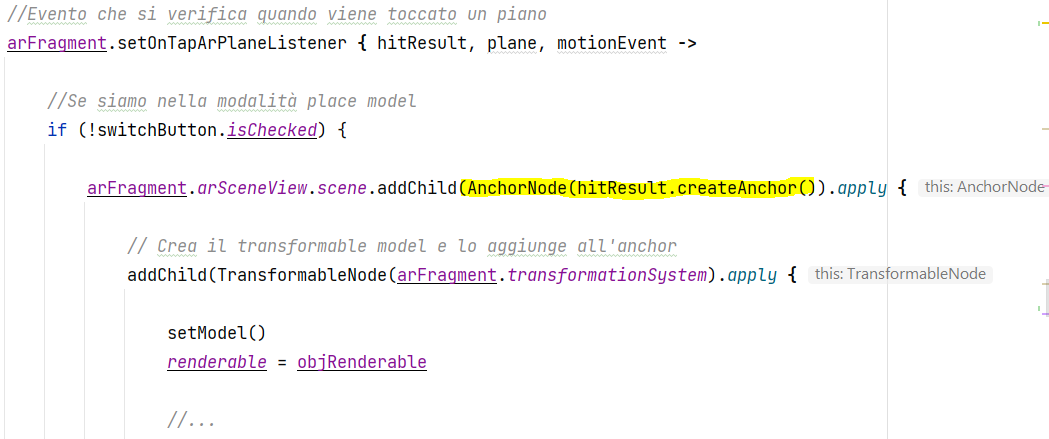
\includegraphics[width=0.9\textwidth]{../../resources/images/UserInteraction/UserInteraction1.PNG}}%
			{Fonte: \url{nostra  applicazione}}
			\caption{Definizione Anchor in Plane Detection}
			\label{fig: Definizione Anchor in Plane Detection}
	\end{figure}
	\vspace{0.2cm}
	\begin{figure}
			\centering
			\copyrightbox[0.5]{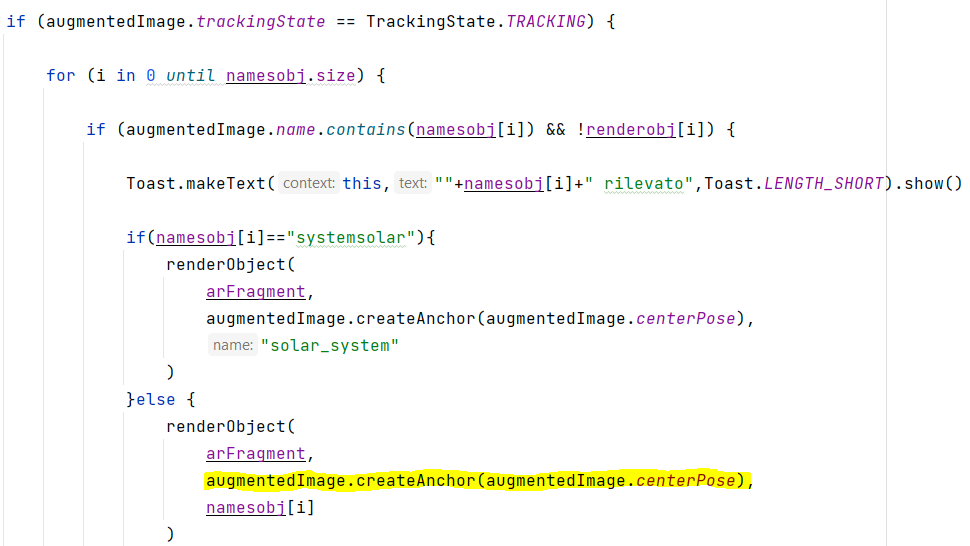
\includegraphics[width=0.9\textwidth]{../../resources/images/UserInteraction/UserInteraction2.PNG}}%
			{Fonte: \url{nostra  applicazione}}
			\caption{Definizione Anchor in Augmented Images}
			\label{fig: Definizione Anchor in Augmented Images}
	\end{figure}
		
		Esistono quattro tipi di risultati che si possono ottenere in una sessione ARCore:
		\begin{itemize}
		\item[•] \textbf{Profondità}: richiede l'attivazione di depth API nella sessione ARCore ed è usato per posizionare oggetti su superfici arbitrarie (non solo su piani).
		\item[•]\textbf{Aereo}: permette di posizionare un oggetto su superfici piane e utilizza la loro geometria per determinare la profondità e l'orientamento del punto individuato.
		\item[•] \textbf{Punto caratteristico}: permette di disporre oggetti in superfici arbitrarie basandosi su caratteristiche visive attorno al punto sul quale l'utente tocca. 
		\item[•] \textbf{Posizionamento istantaneo}: consente di posizionare un oggetto rapidamente in un piano utilizzando la sua geometria completa attorno nel punto selezionato. 
	\end{itemize}
	
	\begin{flushleft}
		Il risultato restituito da hitTest nella modalità \emph{Plane Detection} è di tipo Aereo; il rilevamento di un piano 			consente di disporre un animale in un punto preciso. Questo evento è stato gestito dal metodo 									\textit{setOnTapArPlaneListener} riportato nell'esempio \vref{fig: Definizione Anchor in Plane Detection}.\\
	\end{flushleft}
		
	
\end{document}